\chapter{Felhasználói dokumentáció}
\label{ch:user}


\section{Az alkalmazás célja}

Az alkalmazás célja, hogy a felhasználó segítségével membránrendszereket hozzon létre majd szimulálja számításaikat. A membránrendszer egy olyan biológiailag inspirált számítási modell, amely az eukarióta sejtek működését és felépítését követve evolúciós lépéseken keresztül történő információáramlást ír le membránok között. Minden membrán által körbezárt \textit{ún.} régió tartalmaz evolúciós szabályokat, amelyek nem változnak a membránrendszer működése közben. Az információt a rendszerben a régiókban található molekulák, \textit{ún.} objektumok hordozzák. Egy szabály csak akkor tud végbemenni, ha rendelkezésre állnak a szükséges objektumok kellő számban. Ilyen helyzetekben a szabályoknak végre is kell hajtódnia, tehát nem fordulhat elő, hogy minden objektum hozzáférhető, de nem kerül a szabály alkalmazásra. Egy evolúciós lépésben a maximális párhuzamosság elve érvényesül, azaz a szabályok véletszerűen kerülnek kiválasztása, egészen addig, amíg van alkalmazható szabály. Megadhatóak olyan speciális szamályok, amelyek alkalmazásának hatására egy membrán feloldódhat, ilyenkor a tartalma az őt körbevevő régióba kerül. A szabályok között prioritási sorrend is felállítható. A számítás legfontosabb tulajdonsága annak kimenete, amely általában a legkülső régión kívülre (azaz a környezetbe) kijutó objektumok számát jelenti.


\section{Hardver és szoftver követelmények}

A szoftver futtatásához Linux környezetre van szükség, amely támogatja a \verb|.bin| kiterjesztésű fájlok értelmezését. A program teljes funkcionalitásának kihasználásához a felhasználó számítógépének a bemeneti perifériák közül egérrel és billentyűzettel kell rendelkeznie. A szoftver hardverigénye nem igényel részletesebb specifikációt.


\section{Futtatás}

Mivel a program futtatható állományban kerül a felhasználóhoz, ezért annak az indításhoz elegendő megnyitni a fájlt tartalmazó mappát, majd duplán kattintani a fájlt reprezentáló ikonra. Ugyanez parancssori környezetben is elvégezhető, ilyenkor a terminálban a megfelelő mappába való elnavigálás után a 
\verb|./MembraneSimulator.bin| parancs megadásával futtatható a program.

\section{Grafikus felhasználói felület}

A felhasználó az alkalmazással a grafikus felhasználói felületen keresztül tud kommunikálni, amely a főablakot és az igény szerint megjelenő dialógusablakokat foglalja magába.

\subsection{Főablak}

\begin{figure}[H]
	\centering
	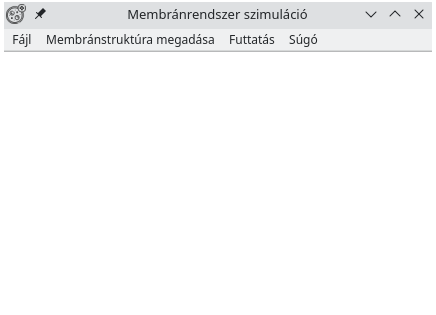
\includegraphics{main_window_empty.png}
	\caption{A főablak az alkalmazás megnyitásakor}
	\label{fig:example-1}
\end{figure}

\subsection{Dialógusablakok}

\subsubsection{Membránstruktúra megadása}
\subsubsection{Objektumok módosítása}
\subsubsection{Szabályok módosítása}
\subsubsection{Szimulációk számának megadása}
\subsubsection{Mentés}
\subsubsection{Betöltés}
\subsubsection{Eredményablak}

\section{Használati útmutató}

